\documentclass{standalone}
\usepackage{pgfplots}
\pgfplotsset{compat=1.18}
\usetikzlibrary{arrows.meta}
\usepgfplotslibrary{fillbetween}

\begin{document}

\definecolor{tab_blue}{HTML}{1F77B4}
\definecolor{tab_orange}{HTML}{FF7F0E}
\definecolor{tab_green}{HTML}{2CA02C}
\definecolor{tab_red}{HTML}{D62728}

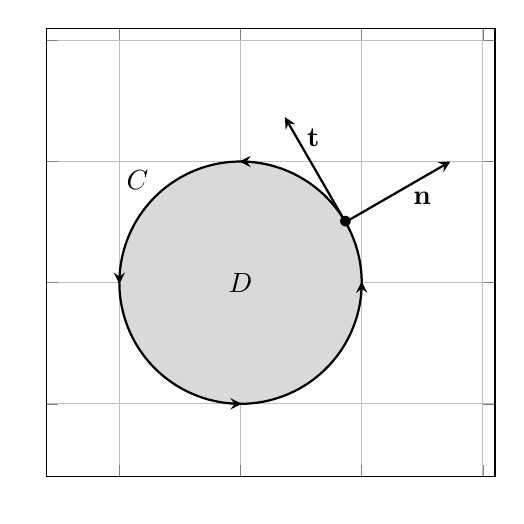
\begin{tikzpicture}
\begin{axis}[
% axis on top,
axis lines = box,
% axis lines = none,
unit vector ratio=1 1, 
% axis equal=false,
scale=1.0, 
xmin=-1.6, xmax=2.1, ymin=-1.6, ymax=2.1, 
xticklabels = {},
yticklabels = {},
grid = major
]

\addplot[domain=0:pi, samples=100, thick, name path=up] ({cos(deg(x))}, {sin(deg(x))}); 
\addplot[domain=pi:2*pi, samples=100, thick, name path=down] ({cos(deg(x))}, {sin(deg(x))}); 
\addplot[fill=gray!30] fill between [of=up and down]; 
\draw[->, >=stealth, thick] (1, 0) -- (1, 0.01);
\draw[->, >=stealth, thick] (0, 1) -- (-0.01, 1);
\draw[->, >=stealth, thick] (-1, 0) -- (-1, -0.01);
\draw[->, >=stealth, thick] (0, -1) -- (0.01, -1);
\node at (-0.85, 0.85) {$C$};
\node at (0, 0) {$D$};
\node at ({sqrt(3)/2}, 1/2) {$\bullet$}; 
\draw[->, >=stealth, thick] ({sqrt(3)/2}, 1/2) -- ({(sqrt(3)-1)/2}, {(sqrt(3)+1)/2});
\draw[->, >=stealth, thick] ({sqrt(3)/2}, 1/2) -- ({sqrt(3)}, 1);
\node at (0.6, 1.2) {$\mathbf{t}$}; 
\node at (1.5, 0.7) {$\mathbf{n}$}; 


\end{axis}
\end{tikzpicture}

\end{document}